\documentclass[submit]{harvardml}

% Put in your full name and email address.
\name{Jian Li, Weiyi Chen, Ethan Cowan}
\email{jil761@g.harvard.edu}

% List any people you worked with.
\collaborators{%
Kaggle team name: L.C.C.
}

% You don't need to change these.
\course{CS181-S16}
\assignment{Practical \#4}
\duedate{11:59pm May 1st, 2016}

\usepackage[OT1]{fontenc}
\usepackage[colorlinks,citecolor=blue,urlcolor=blue]{hyperref}
\usepackage[pdftex]{graphicx}
\usepackage{subfig}
\usepackage{fullpage}
\usepackage{palatino}
\usepackage{mathpazo}
\usepackage{amsmath}
\usepackage{amssymb}
\usepackage{color}
\usepackage{todonotes}
\usepackage{listings}
\usepackage{common}
\usepackage{bm}

\usepackage[mmddyyyy,hhmmss]{datetime}

\definecolor{verbgray}{gray}{0.9}

\lstnewenvironment{csv}{%
  \lstset{backgroundcolor=\color{verbgray},
  frame=single,
  framerule=0pt,
  basicstyle=\ttfamily,
  columns=fullflexible}}{}

\begin{document}
\begin{center}
{\Large Practical 4: Reinforcement Learning}\\
\end{center}

\section{Introduction}
In this practical, we develop a reinforcement learning agent to play Swingy Monkey. In this game, we control a monkey that is trying to swing on vines and avoid tree trunks. We can either make him jump to a new vine, or have him swing down on the vine he’s currently holding. We get points for successfully passing tree trunks without hitting them, falling off the bottom of the screen, or jumping off the top. 

Our objective is to build an agent that learns to play on its own. In our agent, the features are sources of randomness: the monkey’s jumps are sometimes higher than others, the gaps in the trees vary vertically, the gravity varies from game to game, and the distances between the trees are different. We will be using three kinds of methodologies: TD value learning, model based method and Q learning method.

\section{Features or Data}
Based on the rules of this game, we select the following features as our input for TD Value Learning, Model Based Method and Q learning.
\begin{enumerate}
\item The distance to the tree divided by the horizontal speed. After running the game for several epochs, we can observe the horizontal speed remain constant at 25.
\item The vertical location of the money. This feature is used to make sure the monkey doesn't jump or fall out of the screen.
\item The relative vertical position of the monkey with respect to the center of the tree gap.
\item The vertical speed.
\item The gravity. This is not directly observable, but the gravity doesn't change within an epoch, and when there's no jump, gravity is the decrement of the vertical speed in one step, so this is easy to estimate.
\end{enumerate}

\section{Methodologies and Motivations}

\subsection{TD Learning method}

TD learning is temporal difference value learning. 

\subsubsection{Overview and Motivations}
It's a hybrid approach because while it still uses temporal learning update for the value function $V(s)$, we also need to learn we need to learning the transition function $T(s'|s,a)$ and the reward function $R(s,a)$.  
The update equation is
$$V(s) \leftarrow V(s) + \alpha [ (r+\gamma V(s')) - V(s) ]$$
At each step the policy is based on 
$$\pi(s) = argmax_{a\in A} [ R(s,a) + \sum_{s'} P(s'|s,a) V(s') ]$$
where we can use $\epsilon$-greedy exploration on top of this.

\subsubsection{Discretization}
To model the value function based on the five features, we discretize each feature. For example, the vertical location of the monkey we select bin size of monkey height. For relative location of the monkey, we choose half of the monkey height as bin size. 

\subsubsection{Initialization}
The initialization is applying common sense based on the scoring. For example, we set value function to $-10$ when the monkey is close to either the top or the bottom of the screen. We set the value to $-8$ when it's within one monkey height away from boundary but the speed is in the direction towards the boundary. When the tree is far away, we give small value to states where the monkey is in the middle of the screen.

Similarly, when the monkey is close to the tree, we set the value the $-5$ if it will hit the tree, and set value around $1$ if it's close to the center of the tree.

The initialization is reasonable and we see some large scores for earlier epochs sometimes.

\subsubsection{Transition and reward function}
When the monkey is swinging down the transition is actually deterministic. We can easily derive the location of the monkey based on velocity and the velocity is decreasing by the value of the gravity at each step. 

When the monkey jumps, the velocity is randomly chosen. We notice the long term mean slightly above $11$. The vertical position of the monkey will be $y_t + v_{t+1} + g$, where g is gravity. Instead of storing the whole distribution of $v_{jump}$, we use the mean to estimate the state where the monkey will go to, then use the policy to decide whether to jump or not.

The reward function is initialized to zero in the beginning and as sample comes in we will record these scores for future use.

\subsection{Model Based Method}
In this approach we use the dynamics and estimate where the monkey would be in future steps. 

\subsubsection{Motivations}
Because when the monkey doesn't jump, the moves are deterministic, so no additional learning is needed, we can actually calculate where the monkey will be after k steps if it didn't make any jump. Essentially at each step we will decide between two policy set: the first one is to swing down, then continue to swing down in the following steps; the second one is to jump, the swing down in the following steps. When the monkey does jump, we can use its average jump size to estimate its trajectory.

\subsubsection{Rules}
So based on these two sets, we can estimate where the monkey will be when the distance is zero or negative. Within these two policy sets, we consider a $Q(s,a)$ more valuable if it's closer to the center of the tree gap when the distance is zero. So in this model, we use this distance to the tree gap center at the step when distance is zero as our $Q(s,a)$, and take action based on this.

On top of this, when the monkey is far away from the tree (more than 8 steps away), our rule is to choose action to make it closer to the center of the screen, which implies a $Q(s,a)$ with higher values for states closer to the center.

In addition, we notice the gap between the tree is usually 200 so any jump is likely cause it to hit the three. So when distance to the tree is negative, we usually choose not to jump, essentially giving $Q(s,1)$ a lower value than $Q(s,0)$. 

\subsubsection{Note}
In this approach, we don't have to write out $Q(s,a)$ explicitly. The decision making is purely rule based. The caveate is that the model is not very flexible and doesn't take new samples into account and make the policy more adaptive.

\subsection{Q Learning Method}
Q-learning algorithm provides a method to learn the Q function directly without needing to also learn a probabilistic model of the environment. 

\subsubsection{Motivations}
This provides two advantages over model-based approaches: it is no longer necessary to learn a transition model of size $O(N^2M)$ for $N$ states and $M$ actions. Moreover, it avoids the need to perform planning while learning, which can be infeasible in complex domains. On the other hand, we will see that Q-learning can be very slow in terms of the number of periods of experience required to learn a good policy, and much more slow to learn a good policy than model-based RL.

\subsubsection{Overview}
Expanding the definition of the $Q$ function from the Bellman equations, we have
$$ Q(s,a) = E_{s'}\left[ R(s,a) + \gamma \max_{a'\in A} Q(s', a') \right] $$
Our goal then, is to estimate $Q(s,a)$ as the expectation, where $s'$ is drawn from $P(s'\given s,a)$ of $R(s,a) + \max_{a'}Q(s',a)$. But we must do this without having access to the model of the probabilistic transition function.

\subsubsection{Implementation}
This is possible because each time we actually take action $a$ from state $s$ we observe a transition to $s'$ and receive a reward $r$. This gives us a sample from $P(s' \given s, a)$. We can use this sample for updating our old estimate of $Q(s, a)$. Specifically, on transitioning from $s$ to $s'$ under action $a$ and receiving reward $r$, the following update rule used in Q-learning:
$$ Q(s,a) \leftarrow Q(s,a) + \alpha \left[ (r + \gamma \max Q(s',a')) - Q(s,a) \right] $$
where $0<\gamma<1$ is the discount factor and $0<\alpha<1$ is the learning rate.

To get the new estimate of $Q(s, a)$, we move the current estimate by some amount that depends on the error between $Q(s, a)$ and the target value that we find in the new state. The target value is $r + \gamma \max_{a'} Q(s', a')$, which provides a sample of $Q(s, a)$. The rule adjusts towards this, with learning rate $\alpha$ determining how much of an effect the new sample has on the current estimate. If $\alpha$ is large, we will adjust quickly but may not converge. If $\alpha$ is small then we will adjust slowly, but learning may converge. A natural thing to do is to decrease $\alpha$ gradually as the number of samples of $Q(s, a)$ increases.

\section{Implementation and Running Guide}

All of our contribution is enclosed in stub.py file, where the learner class has an argument $algo$ to define which method you would like to use. We have re-implemented \_\_init\_\_() method, action\_callback() method and reset() method inside learner class, also added feat\_normalize() method to normalize features, transition() method for TD learning transition. Please refer to our script regarding our implementation of our methodologies described in section 3.

To run the program, please make sure the main() is defined as below for each method respectively, then "python stub.py" to start - 

\subsection{TD Learning Method Running Guide}
\begin{lstlisting}[language=python]
    # Select agent
    agent = Learner("TD Value")

    # Run game and save history.
    hist = []
    run_games(agent, hist, 200, 1)
    np.save('hist',np.array(hist))
\end{lstlisting}

\subsection{Model Based Method Running Guide}
\begin{lstlisting}[language=python]
    # Select agent
    agent = Learner("Model Based")

    # Run game and save history.
    hist = []
    run_games(agent, hist, 200, 1)
    np.save('hist',np.array(hist))
\end{lstlisting}

\subsection{Q leaning Running Guide}
\begin{lstlisting}[language=python]
    # Select agent
    agent = Learner("qlearn")

    # Run game and save history.
    hist = []
    run_games(agent, hist, 200, 1)
    np.save('hist',np.array(hist))
\end{lstlisting}

\section{Results}

\subsection{TD Learning Method}

We then run the algo and use the update equation for the value function. The results are in Fig. \ref{fig:compare_box}, Fig. \ref{fig:compare_bar} Table \ref{tab:mean} and Table \ref{tab:max}. Initially for the third feature, we choose bin size to be the monkey height and it causes more collision so we used more granular bin size instead. The average score is around 5 when we ran 20 epochs in each test.

\subsection{Model Based Method}
Interestingly, this method gave very good results, compared with TD Value learning. As seen in Fig. \ref{fig:compare_box}, there's one epoch it got score more than 300. There's another one it got 180. This shows that expert knowledge (the dynamics of the move as understood by human) can make even a simple system very effective.  

\subsection{Q Learning Method}
As expected from our motivation, Q learning turns out the best results, compared to the former two methods. As seen in Fig. \ref{fig:compare_box}, \ref{fig:compare_bar} the max score even reaches 2212 (see Fig. \ref{fig:screenshot}), and either its max or min score is stably higher than the other methods. This reverts the conclusion of the previous part that learning algorithm is more able to capture the system more effective compared to dynamics move by human because it is able to do more detailedly and provide more storage space.
 
\begin{figure}[htbp]
\centering
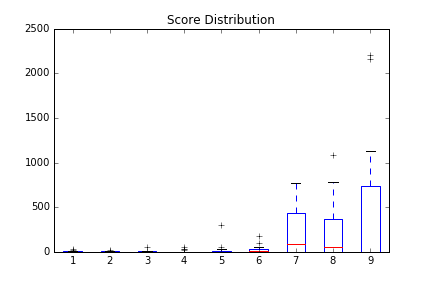
\includegraphics[width=0.6\textwidth]{box_comparison.png}
\caption{Score distribution comparison: 1-3 use TD Value Learning, and correspond to test 1-3 in the score table. 4-6 use model based approach and correspond to test 1-3 of model based method in the score table. 7-9 use Q learning method and correspond to test 1-3 of Q learning method in the score table. }
\label{fig:compare_box}
\end{figure}

\begin{figure}[htbp]
\centering
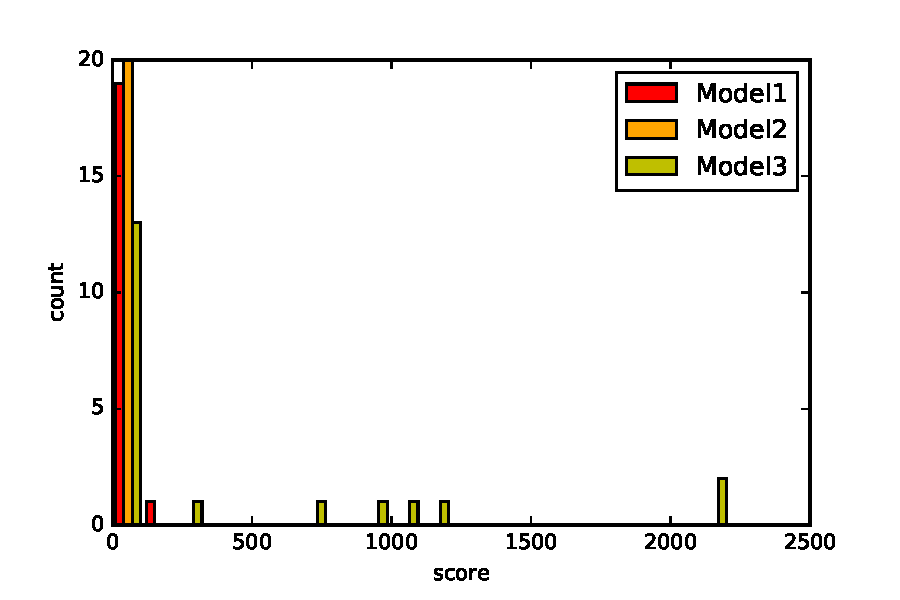
\includegraphics[width=0.6\textwidth]{bar_comparison.pdf}
\caption{Score distribution histogram comparison: Model 1 use TD Value Learning, and correspond to test 3 in the score table. Model 2 use model based approach and correspond to test 3 of model based method in the score table. Model 3 use Q learning method and correspond to test 3 of Q learning method in the score table. }
\label{fig:compare_bar}
\end{figure}

\begin{figure}[htbp]
\centering
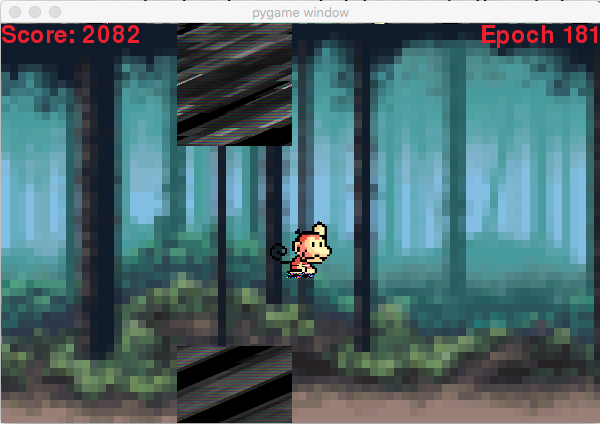
\includegraphics[width=0.6\textwidth]{screenshot}
\caption{Screenshot of a game with high score}
\label{fig:screenshot}
\end{figure}

\begin{table}
\begin{center}
  \begin{tabular}{ | l | l | l | l  | }
    \hline
		Method & Test 1 & Test 2 & Test 3 \\ \hline
TD Value &		 4.75 &   5.6 &   6.5 \\ \hline   
Model Based &		7.55 &  24.15 &  25.7 \\ \hline		
Q Learning &   241.1 & 208.7 & 426.1 \\ \hline
  \end{tabular}
\end{center}
\caption{Average score of three tests for three methods}
\label{tab:mean}
\end{table}

\begin{table}
\begin{center}
  \begin{tabular}{ | l | l | l | l  | }
    \hline
    Method & Test 1 & Test 2 & Test 3 \\ \hline
TD Value &     32 &   46 &   58 \\ \hline   
Model Based &   56 &  308 &  182 \\ \hline   
Q Learning &   776 & 1091 & 2212 \\ \hline
  \end{tabular}
\end{center}
\caption{Max score of three tests for three methods}
\label{tab:max}
\end{table}

\section{Conclusion}
In this practical, we developed a reinforcement learning agent which contains three methods to play Swingy Monkey. Among three methods in our agent, they are sharing the same features, as of the monkey’s jumps are sometimes higher than others, the gaps in the trees vary vertically, the gravity varies from game to game, and the distances between the trees are different. 

Through the comparison between model based approach and TD learning method, we drew the conclusion that expert knowledge (the dynamics of the move as understood by human) can make even a simple system very effective, as a simple implemented model based approach can turn out a better result than TD learning. However, through the comparison betweern model based approach and Q learning method, we figured out if given more time/epochs to train the model, Q learning algorithm is more capable to capture the system more effectively, because it is able to do more detailedly and provide more storage space.

Via this practical, we realize the advantages of Q learning. It is no longer necessary to learn a transition model of size $O(N^2M)$ for $N$ states and $M$ actions, as TD learning method does. Moreover, it avoids the need to perform planning while learning, which can be infeasible in complex domains. These are all very helpful in our experiments. 

\end{document}
